\chapter{Application}\label{app}
Now, let us have a look how this thesis was conducted after studied thoroughly the related works and the theoretical backgrounds. In following, we will first apply the odometry method by using the rotary encoder. After that, we will proceed by implementing EKF which is available in the Robot Operating System (ROS) library. In this part, we will see which parameter is used and their relation to each other. Following that, we will apply two different scan registration method which is NDT and ICP. As last thing which is the main contribution of the thesis that we will combine all these there different approaches to obtain more robust localization and fully utilize every available sensor on the system.

\section{Wheel Odometry}
Wheel odometry node\footnote{It can simply be thought an executable file in ROS package} receives the wheel displacement and steering angle information from sensors to calculate the displacement of the vehicle in a certain time slot. As consequence, the note delivers pose and velocity information in local frame as well as heading angle and its rate.
\\
\par The odomety algorithm uses the well-know kinetic equations to populates output of the node as follows.
\begin{align}
    &V_{left} = \Delta X_L*D_n/ \Delta t\\
    &V_{right} = \Delta X_R*D_n/ \Delta t\\
    &V_x = (V_{left}+V_{right})/2\\
    &R = wheelbase/sin(\alpha)\\
    &\phi = V_x * \Delta t / R\\
    &x \leftarrow x+\Delta x, \hspace{5pt} \Delta x = R * sin(\phi)\\
    &y \leftarrow y+\Delta y, \hspace{5pt} \Delta y = -(R-R*cos(\phi))
\end{align}
where $V_{left/right}$ are and velocity of left and right wheel respectively, which are calculated over elapsed time $\Delta t$. $\alpha$ is steering angle which is provided by steering wheel for calculating $\phi$ is heading angle and as a last,  position of the vehicle is estimated in direction of $x$ and $y$ in local frame by using turning radius $R$ which depends on steering angle $\alpha$ and difference between front and rear wheel $wheelbase$.\\
%we can easily derive displacement of the car over time in equation:
\begin{figure}[H]
    \begin{subfigure}{.5\textwidth}
        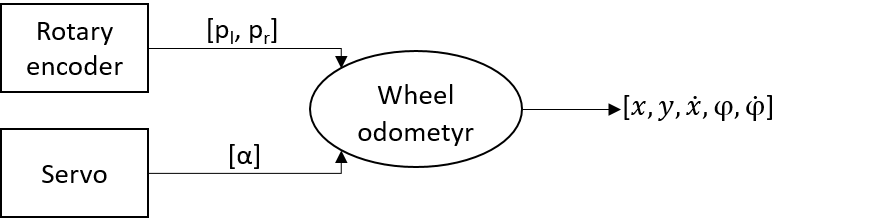
\includegraphics[scale=0.5]{odom_node}
        \label{fig:odom_pose}
    \end{subfigure}
    \begin{subfigure}{.5\textwidth}
        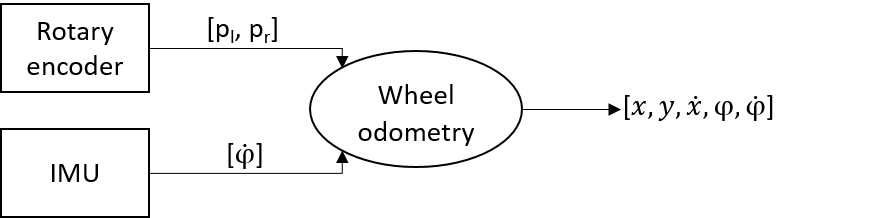
\includegraphics[scale=0.5]{odom_node_imu}
        \label{fig:odom_pose_imu}
    \end{subfigure}
    \caption{Wheel Odometry Node}
    \label{fig:odometry}
\end{figure}
\noindent Please note that, we assume there is no movement w.r.t roll, pitch angle and Z direction. Addition to this, there is not any velocity component in direction of y is "0" since the vehicle unable to catch any lateral force. Additionally, we calculating odometry in two different ways as shown in Figure \ref{fig:odometry}. First, we calculate the heading angle and rate using steering angle. Second, we use the IMU to get directly these two values without performing any mathematical effort. The result of these two approaches is presented in following section.

\section{Extended Kalman Filter}
In this section, the task is fusing IMU and odometry data. As mention in the previous chapter, we immigrate the EKF from ROS library into this thesis. Therefore, we have to only decide that which state we would like to estimate and what are our observation data from sensors. To proceed with EKF, we first introduce what state we can estimate and how we configure them in state estimation node \cite{kalman7}. In this node, the vehicle can be track in 15 different dimension like position, velocity and acceleration in 3D Cartesian coordinate system and in Euler angles as well as their rates as follows:
\begin{equation}\label{eq:state}
 \begin{bmatrix}
X & Y &Z\\
roll& pitch& yaw&\\
\dot X & \dot Y& \dot Z\\
\dot {roll} & \dot {pitch}& \dot {yaw}\\
\ddot X & \ddot Y& \ddot Z
\end{bmatrix}   
\end{equation}
\par In configuration phase, we should decide which parameter should be fused. As shown in figure \ref{fig:odometry}, the odometry node provides x, y position in the local reference frame, velocity and heading rate in the body frame, while IMU provides heading rates and linear acceleration in body frame w.r.t roll, pitch, yaw and x, y, z respectively.
\\
\begin{figure}[H]
    \centering
    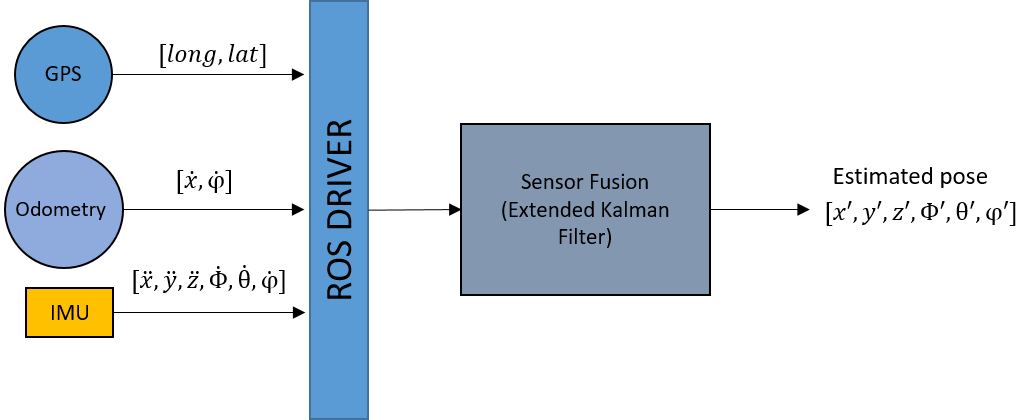
\includegraphics[width=\textwidth,height=6cm]{ekf.png}
    \caption{Caption}
    \label{fig:ekf_node}
\end{figure}
\newpage
We fuse the velocity and heading rate provided by odometry node along IMU data into state estimate node. It is important to note that, we do not fuse x, y parameter of odometry as long as IMU exist on the system. The reason is only avoiding to duplicate information since the velocity and absolute position of the vehicle calculated from the same source that may cause the filter to diverge from the desired value. You may also wonder why do we fuse the y component of the velocity ($\dot Y$), in spite of being mentioned as "0" at beginning of this chapter. At first glance, it does not make sense but it actually helps the filter to infer that there is no movement in the y-direction. At the end we have configuration matrix for every single sensor as follows:
\\
\begin{equation}\label{eq:config}
    \begin{bmatrix}
    false,&false,&false\\
    false,&false,&false\\
    true,&true,&false\\
    false,&false,&true\\
    false,&false,&false
    \end{bmatrix}
\end{equation}\\

\noindent where \textbf{\textit{false}} means the value will not be fuse while \textbf{\textit{true}} means the value will be fused. Note that the matrix in equation \eqref{eq:config} maps the matrix in equation \eqref{eq:state}

\par As a next and last step, we should tune the process and measurement noise co-variance matrices \textbf {Q} and \textbf{P},respectively. These two matrices are 15 by 15 size, diagonal and all its elements regard to state matrix. Here, the rule we should follow for setting \textbf {Q} and \textbf{P}: Assume that we would like tune EKF for one measuring parameter, so we have to change the value of the diagonal variable that corresponds to be fused parameter in Q and P matrix. Thus, we can influence the filter in a way that changes its fast to converge true value. For instance, if one can set the diagonal value of P matrix for velocity ($\dot X$) bigger than that measurement’s co-variance so, it makes the filter converge faster. On the other hand, if one can increase the diagonal value of Q matrix and hence it causes the error to grow faster in the state estimate part. Therefore, it effect filter converge faster in principle. However, it is very hard to tune both Q and P matrices but one can reach very optimal result by tuning them. In chapter \ref{sec:result}, it shows the affect of P and Q on EKF.

\section{Normal Distribution Transform}
This section, we describe how NDT method is applied in order to estimate pose in 6 degrees of freedom (DOF). This application is improved by pulling it from point clouds (PCL) and Autoware which are both open source libraries. The basic NDT algorithm is designed to use only point clouds information for finding  most likelihood transformation between the reference and target model as shown in figure \ref{fig:ndt}.
\begin{figure}[H]
    \centering
    \setlength{\fboxsep}{0pt}%
    \setlength{\fboxrule}{1pt}%
    \fbox{
    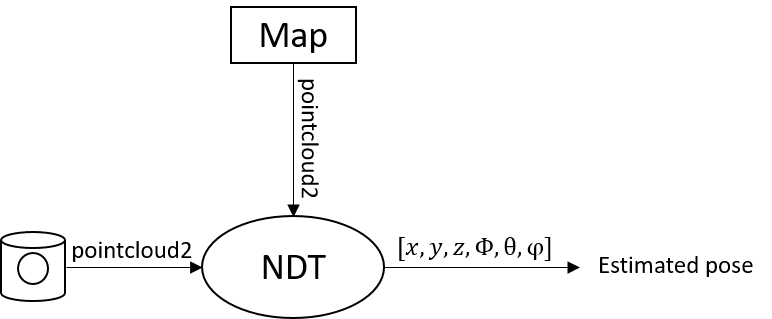
\includegraphics[scale=0.6]{ndt}}
    \caption{Workt Flow of the basic NDT algorithm} 
    \label{fig:ndt}
\end{figure}
NDT tries to extract the position of vehicle on the prior map. However, the basic NDT has a tendency to lose track of position against any disturbance for example, change of environment conditions. Therefore, we first link the odometry reading with NDT in order to support for tracking pose. We here note that we are not using position of odometry since it is not only prone to drift but also it uses different frame than NDT. Due to the fact, only the linear and angular velocity of odometry is used to recalculate the relative position. After that, the found position is added to the current position for correcting the estimated position of NDT. Subsequently, NDT node is redesigned as shown in figure \ref{fig:ndt_odom}.
\begin{figure}[H]
    \centering
    \setlength{\fboxsep}{0pt}%
    \setlength{\fboxrule}{1pt}%
    \fbox{
    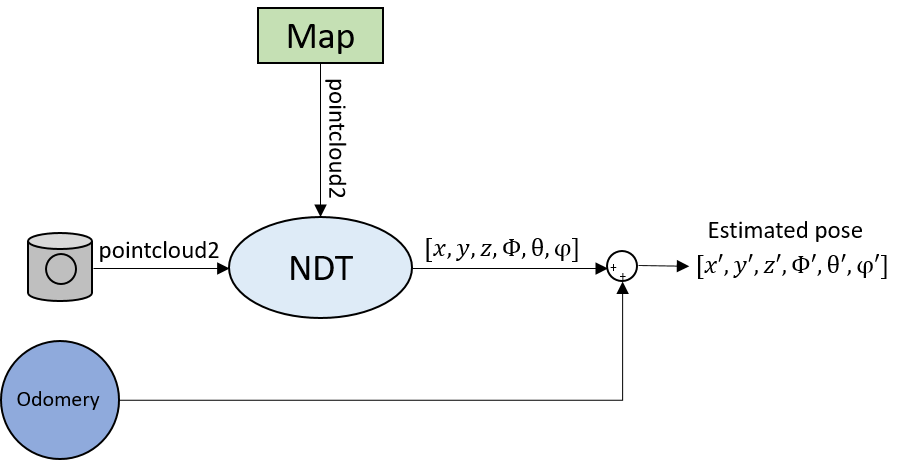
\includegraphics[scale=0.6]{ndt_odom}}
    \caption{Caption}
    \label{fig:ndt_odom}
\end{figure}
\par However, a further improvement of NDT is needed since odomerty has lack of information about the movement of vehicle and it is unreliable for long-term localization as we discussed in section \ref{sec:odom}. At this point, EKF is brought into play to support the algorithm in order to make it more robust. We employ EKF with odometry and IMU data to add NDT as shown in figure \ref{fig:ndt_ekf}.
\begin{figure}
    \centering
    \setlength{\fboxsep}{0pt}%
    \setlength{\fboxrule}{1pt}%
    \fbox{
    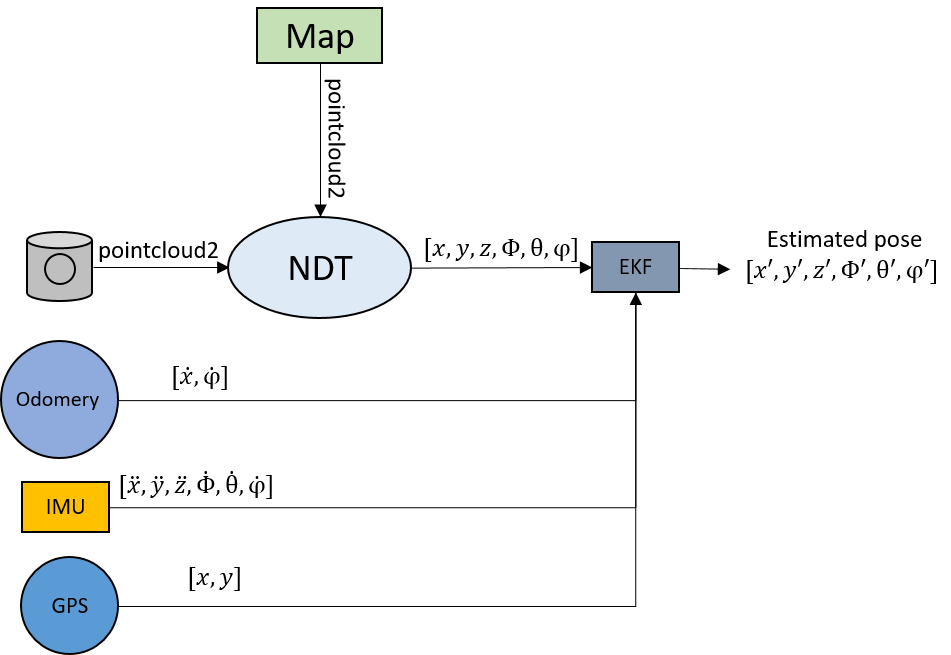
\includegraphics[scale=0.52]{ndt_ekf}}
    \caption{Caption}
    \label{fig:ndt_ekf}
\end{figure}
The advantage of employing EKF in this fashion is improving the result and removing the noise from sensors.
\par Yet there is another derivation of this application- In this instance, we use two EKF. One is used in the same way as the previous one. The other one is used for fusing NDT, IMU, and odometry as shown in figure \ref{fig:ndt_2ekf}. The purpose of doing this is eliminating unwanted movement of NDT since it estimates the pose of the vehicle in map frame hence it generates discrete jumps in a time period even though it eliminates drift \cite{rep105}. 
\begin{figure}[H]
    \centering
    \setlength{\fboxsep}{0pt}%
    \setlength{\fboxrule}{1pt}%
    \fbox{
    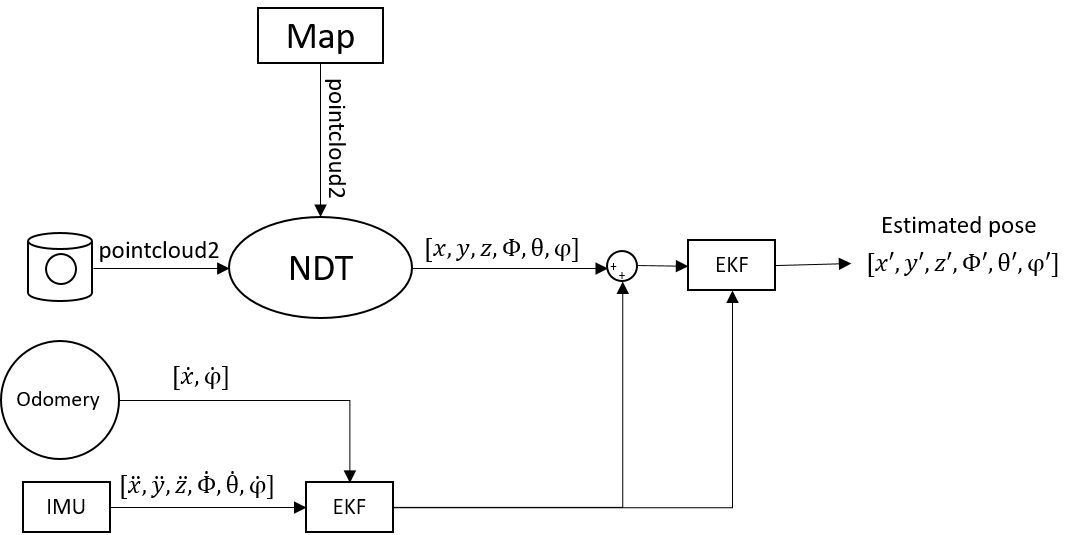
\includegraphics[scale=0.52]{ndt_2ekf}}
    \caption{Caption}
    \label{fig:ndt_2ekf}
\end{figure}

\par On the other hand, the algorithm is still not capable of self initialization. As mentioned in section \ref{sec:summary} is that NDT and ICP cannot find the matches between two scans unless they do know where to start. Therefore, we should provide a initial transform between the vehicle and the map. Thus, we approach this problem from GPS perspective. First, we provide static transformation between map and local coordinate by converting the first GPS output longitude and latitude, where a map is started to build, to Universal Transverse Mercator (UTM) coordinate by using geodetic tool \cite{utm}. Now, we have two transformations which are from GPS to map $_{M}^{G}T$ and GPS to vehicle $_{V}^{G}T$. Next step is finding transformation between map and vehicle $_{M}^{V}T$ by using chain rule property as follows \cite{robotic}:
\begin{align}
    _{M}^{G}T &= _{V}^{G}T \cdot _{M}^{V}T\\
    _{M}^{V}T &= _{V}^{G}T \cdot _{M}^{G}T^{-1}
\end{align}
It should be noted that the heading angle of the vehicle is provided from IMU for finding transformation  $_{M}^{V}T$ since GPS provides only longitude and latitude information.
\\
\par As a result of these improvements, NDT is transformed into a more robust algorithm than basic NDT as shown in figure \ref{fig:ndt_son}. Hence, NDT becomes more versatile to answer "where am I" and "where am I going" fundamental questions of robot navigation.  
\begin{figure}[H]
    \centering
    \setlength{\fboxsep}{0pt}%
    \setlength{\fboxrule}{1pt}%
    \fbox{
    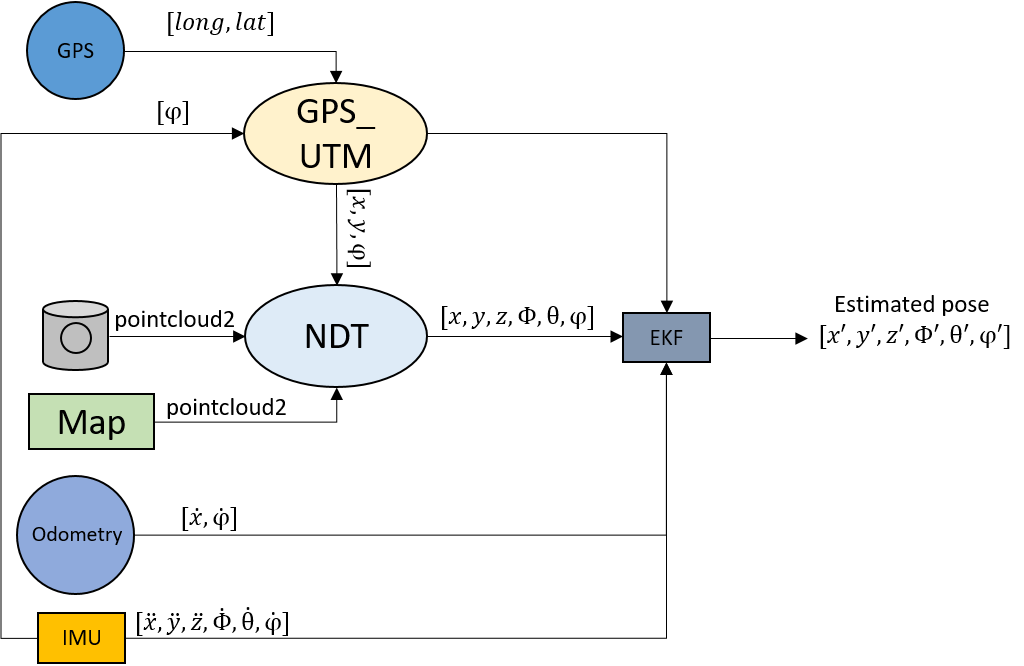
\includegraphics[scale=0.5]{ndt_son}}
    \caption{Caption}
    \label{fig:ndt_son}
\end{figure}
\section{Iterative Closest Points}